%%% The main file. It contains definitions of basic parameters and includes all other parts.

%% Settings for single-side (simplex) printing
% Margins: left 40mm, right 25mm, top and bottom 25mm
% (but beware, LaTeX adds 1in implicitly)
\documentclass[12pt,a4paper]{report}
\setlength\textwidth{145mm}
\setlength\textheight{247mm}
\setlength\oddsidemargin{15mm}
\setlength\evensidemargin{15mm}
\setlength\topmargin{0mm}
\setlength\headsep{0mm}
\setlength\headheight{0mm}
% \openright makes the following text appear on a right-hand page
\let\openright=\clearpage

%% Settings for two-sided (duplex) printing
% \documentclass[12pt,a4paper,twoside,openright]{report}
% \setlength\textwidth{145mm}
% \setlength\textheight{247mm}
% \setlength\oddsidemargin{14.2mm}
% \setlength\evensidemargin{0mm}
% \setlength\topmargin{0mm}
% \setlength\headsep{0mm}
% \setlength\headheight{0mm}
% \let\openright=\cleardoublepage

%% Generate PDF/A-2u
\usepackage[a-2u]{pdfx}

%% Character encoding: usually latin2, cp1250 or utf8:
\usepackage[utf8]{inputenc}

%% Prefer Latin Modern fonts
\usepackage{lmodern}

%% Further useful packages (included in most LaTeX distributions)
\usepackage{amsmath}        % extensions for typesetting of math
\usepackage{amsfonts}       % math fonts
\usepackage{amsthm}         % theorems, definitions, etc.
\usepackage{bbding}         % various symbols (squares, asterisks, scissors, ...)
\usepackage{bm}             % boldface symbols (\bm)
\usepackage{graphicx}       % embedding of pictures
\usepackage{fancyvrb}       % improved verbatim environment
\usepackage[numbers]{natbib}         % citation style AUTHOR (YEAR), or AUTHOR [NUMBER]
\usepackage[nottoc]{tocbibind} % makes sure that bibliography and the lists
			    % of figures/tables are included in the table
			    % of contents
\usepackage{dcolumn}        % improved alignment of table columns
\usepackage{booktabs}       % improved horizontal lines in tables
\usepackage{paralist}       % improved enumerate and itemize
\usepackage{xcolor}         % typesetting in color
\usepackage[textsize=tiny]{todonotes}
\usepackage{algorithm}
\usepackage{algpseudocode}



\reversemarginpar
%%% Basic information on the thesis

% Thesis title in English (exactly as in the formal assignment)
\def\ThesisTitle{Optimal choice of scenario tree using Reinforcement learning}

% Author of the thesis
\def\ThesisAuthor{Bc. Jakub Vondráček}

% Year when the thesis is submitted
\def\YearSubmitted{2022}

% Name of the department or institute, where the work was officially assigned
% (according to the Organizational Structure of MFF UK in English,
% or a full name of a department outside MFF)
\def\Department{Department of Probability and Mathematical Statistics}

% Is it a department (katedra), or an institute (ústav)?
\def\DeptType{Department}

% Thesis supervisor: name, surname and titles
\def\Supervisor{doc.~RNDr.~Ing.~Miloš~Kopa,~Ph.D.}

% Supervisor's department (again according to Organizational structure of MFF)
\def\SupervisorsDepartment{Department of Probability and Mathematical Statistics}

% Study programme and specialization
\def\StudyProgramme{Probability, mathematical statistics and econometrics}
\def\StudyBranch{\textcolor{red}{study branch}}

% An optional dedication: you can thank whomever you wish (your supervisor,
% consultant, a person who lent the software, etc.)
\def\Dedication{%
I am infinitely grateful to my supervisor doc.~RNDr.~Ing.~Miloš~Kopa,~Ph.D. for his expertise, patience and all the time and effort spent supervising my thesis. I also thank my consultant RNDr.~Karel~Kozmík for always being ready to help whenever I needed guidance and infinitely many great ideas and suggestions.

I dedicate this thesis to my grandmother and my mother, as without them, I would be nowhere near as far along in life as I am today. Thank you.
}

% Abstract (recommended length around 80-200 words; this is not a copy of your thesis assignment!)
\def\Abstract{%
Abstract.
}

% 3 to 5 keywords (recommended), each enclosed in curly braces
	\def\Keywords{%
{Stochastic optimization}, {Multistage problem}, {Reinforcement learning}
}

%% The hyperref package for clickable links in PDF and also for storing
%% metadata to PDF (including the table of contents).
%% Most settings are pre-set by the pdfx package.
\hypersetup{unicode}
\hypersetup{breaklinks=true}

% Definitions of macros (see description inside)
%%% This file contains definitions of various useful macros and environments %%%
%%% Please add more macros here instead of cluttering other files with them. %%%

%%% Minor tweaks of style

% These macros employ a little dirty trick to convince LaTeX to typeset
% chapter headings sanely, without lots of empty space above them.
% Feel free to ignore.
\makeatletter
\def\@makechapterhead#1{
  {\parindent \z@ \raggedright \normalfont
   \Huge\bfseries \thechapter. #1
   \par\nobreak
   \vskip 20\p@
}}
\def\@makeschapterhead#1{
  {\parindent \z@ \raggedright \normalfont
   \Huge\bfseries #1
   \par\nobreak
   \vskip 20\p@
}}
\makeatother

% This macro defines a chapter, which is not numbered, but is included
% in the table of contents.
\def\chapwithtoc#1{
\chapter*{#1}
\addcontentsline{toc}{chapter}{#1}
}

% Draw black "slugs" whenever a line overflows, so that we can spot it easily.
\overfullrule=1mm

%%% Macros for definitions, theorems, claims, examples, ... (requires amsthm package)

\theoremstyle{plain}
\newtheorem{thm}{Theorem}
\newtheorem{lemma}[thm]{Lemma}
\newtheorem{claim}[thm]{Claim}

\theoremstyle{plain}
\newtheorem{defn}{Definition}

\theoremstyle{remark}
\newtheorem*{cor}{Corollary}
\newtheorem*{rem}{Remark}
\newtheorem*{example}{Example}

%%% An environment for proofs

\newenvironment{myproof}{
  \par\medskip\noindent
  \textit{Proof}.
}{
\newline
\rightline{$\qedsymbol$}
}

%%% An environment for typesetting of program code and input/output
%%% of programs. (Requires the fancyvrb package -- fancy verbatim.)

\DefineVerbatimEnvironment{code}{Verbatim}{fontsize=\small, frame=single}

%%% The field of all real and natural numbers
\newcommand{\R}{\mathbb{R}}
\newcommand{\N}{\mathbb{N}}

%%% Useful operators for statistics and probability
\DeclareMathOperator{\pr}{\textsf{P}}
\DeclareMathOperator{\E}{\textsf{E}\,}
\DeclareMathOperator{\var}{\textrm{var}}
\DeclareMathOperator{\sd}{\textrm{sd}}

%%% Transposition of a vector/matrix
\newcommand{\T}[1]{#1^\top}

%%% Various math goodies
\newcommand{\goto}{\rightarrow}
\newcommand{\gotop}{\stackrel{P}{\longrightarrow}}
\newcommand{\maon}[1]{o(n^{#1})}
\newcommand{\abs}[1]{\left|{#1}\right|}
\newcommand{\dint}{\int_0^\tau\!\!\int_0^\tau}
\newcommand{\isqr}[1]{\frac{1}{\sqrt{#1}}}

%%% Various table goodies
\newcommand{\pulrad}[1]{\raisebox{1.5ex}[0pt]{#1}}
\newcommand{\mc}[1]{\multicolumn{1}{c}{#1}}


\usepackage{sectsty}
\allsectionsfont{\raggedright}

\renewcommand*{\cite}{\citet}

% Title page and various mandatory informational pages
\begin{document}
%%% Title page of the thesis and other mandatory pages
%%% Title page of the thesis

\pagestyle{empty}
\hypersetup{pageanchor=false}
\begin{center}

\centerline{\mbox{
\includegraphics[width=166mm]{../img/logo-en.pdf}}}

\vspace{-8mm}
\vfill

{\bf\Large MASTER THESIS}

\vfill

{\LARGE\ThesisAuthor}

\vspace{15mm}

{\LARGE\bfseries\ThesisTitle}

\vfill

\Department

\vfill

{
\centerline{\vbox{\halign{\hbox to 0.45\hsize{\hfil #}&\hskip 0.5em\parbox[t]{0.45\hsize}{\raggedright #}\cr
Supervisor of the master thesis:&\Supervisor \cr
\noalign{\vspace{2mm}}
Study programme:&\StudyProgramme \cr
\noalign{\vspace{2mm}}
Study branch:&\StudyBranch \cr
}}}}


\vfill

% Zde doplňte rok
Prague \YearSubmitted

\end{center}

\newpage

%%% Here should be a bound sheet included -- a signed copy of the "master
%%% thesis assignment". This assignment is NOT a part of the electronic
%%% version of the thesis. DO NOT SCAN.

%%% A page with a solemn declaration to the master thesis

\openright
\hypersetup{pageanchor=true}
\pagestyle{plain}
\pagenumbering{roman}
\vglue 0pt plus 1fill

\noindent
I declare that I carried out this master thesis independently, and only with the cited
sources, literature and other professional sources. It has not been used to obtain another
or the same degree.

\medskip\noindent
I understand that my work relates to the rights and obligations under the Act No.~121/2000 Sb.,
the Copyright Act, as amended, in particular the fact that the Charles
University has the right to conclude a license agreement on the use of this
work as a school work pursuant to Section 60 subsection 1 of the Copyright~Act.

\vspace{10mm}

\hbox{\hbox to 0.5\hsize{%
In \hbox to 6em{\dotfill} date \hbox to 6em{\dotfill}
\hss}\hbox to 0.5\hsize{\dotfill\quad}}
\smallskip
\hbox{\hbox to 0.5\hsize{}\hbox to 0.5\hsize{\hfil Author's signature\hfil}}

\vspace{20mm}
\newpage

%%% Dedication

\openright

\noindent
\Dedication

\newpage

%%% Mandatory information page of the thesis

\openright

\vbox to 0.5\vsize{
\setlength\parindent{0mm}
\setlength\parskip{5mm}

Title:
\ThesisTitle

Author:
\ThesisAuthor

\DeptType:
\Department

Supervisor:
\Supervisor, \SupervisorsDepartment

Abstract:
\Abstract

Keywords:
\Keywords

\vss}

\newpage

\openright
\pagestyle{plain}
\pagenumbering{arabic}
\setcounter{page}{1}


%%% A page with automatically generated table of contents of the master thesis

\tableofcontents

%%% Each chapter is kept in a separate file
\chapter*{Introduction}
\addcontentsline{toc}{chapter}{Introduction}
Stochastic programming is a branch of mathematical optimization that allows to account for uncertain parameters when solving mathematical programs, which led to the widespread adoption of stochastic programming in fields such as finance, transportation, scheduling and telecommunications. 

This makes it a very powerful tool, which however comes at a significant computational cost. Due to the fact that the random parameters may follow a continuous distribution, approximating such distributions by a discrete set of scenarios is necessary to even be able to formulate the model and also to be able to solve it in finite time. Even more demanding are so called multistage programs, which allow multiple decision periods. To be able to solve multistage programs, the scenarios approximating the continuous distributions in every stage are arranged in a scenario tree. The structure of this tree is very important for the obtained solution, as a tree that is very simple may not approximate the underlying distribution correctly, while a tree that is too complex suffers from extensive computational costs. 

This is the main idea of this thesis -- to discover whether it is possible to predict a scenario tree structure that is optimal with regard to the objective function and also potentially with regard to the complexity of the scenario tree. To solve this problem, we propose an experiment to train a reinforcement learning agent using the solutions of a mean-CVaR model calculated using scenario trees generated from historical financial data. 

Chapters \ref{chap1}, \ref{chap2} and \ref{chapter3} provide the necessary theory for Multistage stochastic programming, the mean CVaR model and Reinforcement learning respectively. The mean CVaR model formulated in Section \ref{section:endofhorizoncvar_scenario_formulation}, while certainly not novel, is of our own design.  The main contribution of this thesis is Chapter \ref{chapter4}, the pinnacle of this thesis, where we implement the experiment described above and analyse the results. To the best of our knowledge, such an experiment has not been proposed in the literature. Also a notable contribution is the compilation and standardization of notation for several machine learning algorithms in Chapter \ref{chapter3} from multiple different sources.
\chapter{Stochastic programming}


%
%Structure of thesis:
%Introduction
%Multistage stochastic programming problems
%-multistage idea, nonanticipativity constraints, deterministic equivalent
%-curse of dimensionality
%-scenario trees 
%    -moment matching, geometric brownian motion + clustering
%Risk measures
%-VaR, CVaR, minimisation, L shaped method, reformulating as a multistage program
%Reinforcement learning
%-introduction, comparison to other types (supervised etc), no loss function - inspiration from learning of animals and men
%-Basic idea
%-Multiarmed bandits
%Study
%-Formulation of the whole problem (idea of thesis)
%    -Idea how to evaluate
%    -Penalisation of result using complexity of tree with a hyperparameter - explain reasoning why we should penalise the result - why are complex scenario trees bad (long computation time, ...)?
%-Data
%-Computational problems, complexity, how long does solving each small problem take
%-Results of the study
%

%Stochastic programming 
%-Framework to model problems which involve uncertainty
%-Optimization problem where some or all parameters are uncertain in contrast to deterministic optimization
%-the goal is to find a solution which is feasible for all such data and optimal in some sense
%-Stochastic programming models are similar in style but take advantage of the fact that probability distributions governing the data are known or can be estimated
%-The goal is to find some policy that is feasible for all (or almost all) the possible parameter realizations
%and optimizes the expectation of some function of the decisions and the random variables
%-Areas where stochastic programming is used
%	-financial planning, airline scheduling, transportation (truck routes, daily milk delivery with random demand), management of power systems
	
In this chapter, we give an introduction to the theory of stochastic programming with particular focus on multistage linear programs. Most of the content in this chapter is based on the material covered in \cite[Chapter 1]{stochasticprogrammingbible}, \cite[Chapters 1-3]{stochasticprogrammingbible2009} and \cite[Part 2]{dupacovastochasticprogramming}.
\todo{Add more meat here}

\section{Basic definitions}
\begin{defn}{Mathematical program in $\R^n$ \cite[p. 107]{dupacovastochasticprogramming}}. \\
\label{def:MathematicalProgramDef}
Let $p,m,n \in \N$. A mathematical program in $\R^n$ is defined as
\begin{equation*}
\mathrm{min} \{f(\mathbf{x}), \mathbf{x} \in \mathbf{M}\},
\end{equation*}
where $\mathbf{M} \subset \R^n$ and $f$ is a real function. The function $f$ is called the objective function and the set $\mathbf{M}$ is called the set of feasible solutions. 
This set is usually defined by constraints as follows:
\begin{equation*}
	\mathbf{M} = \{\mathbf{x} \in \R^n: h_j(\mathbf{x})=0, \, j=1,\dots,p, \, g_k(\mathbf{x}) \leq 0, k=1,\dots,m \},
\end{equation*}
where $h_j,j=1,\dots,p$ and $g_k, k=1,\dots,m $ are real functions.
\end{defn}
If $\mathbf{M}=\R^n$ and all functions in Definition~\ref{def:MathematicalProgramDef} are linear, we call the problem a \textit{Linear program}.
Furthermore, if any of the functions mentioned in Definition~\ref{def:MathematicalProgramDef} depend on parameters, we call the problem a \textit{Parametric program}. If any of the parameters are uncertain \textcolor{red}{(random variables)}\todo{Is random variable ok here? I assume it is, just for check.}, we call the problem a \textit{Stochastic program}.


However, the Stochastic program is not well defined. Consider the Definition~\ref{def:MathematicalProgramDef} and let $\Omega$ be a non-empty set, $\mathcal{F}$ be a  $\sigma$-algebra on $\Omega$, $\omega \in \Omega$ and $\mathcal{P}$ be a probability measure on $(\Omega, \mathcal{F})$, leading to a probability space $(\Omega, \mathcal{F}, \mathcal{P})$. In the context of a Stochastic program, the function $f$ does not depend on $\mathbf{x}$ only, but also on the realisation of $\omega$. This leads to a nonsensical definition, as for different realisations of $\omega$, the optimal value may be different. The standard way to handle this problem is to consider minimisation of expected value of the function $f$:

\begin{equation*}
\mathrm{min} \{\mathbb{E}\left[f(\mathbf{x}, \omega)\right], \mathbf{x} \in \mathbf{M}\},
\end{equation*}
where $\mathbb{E}$ is the expected value operator defined with respect to the probability measure $\mathcal{P}$. \todo{Are these definitions (mostly the probability measure stuff) correct?}


\section{Multistage stochastic programming}
The stochastic programming paradigm allows to make an optimal decision with regard to the expectation, but only for one decision period. This is a considerable limitation, which can be overcome by extending the notion of a \textit{Stochastic program} to a \textit{Multistage stochastic program}. 

\subsection{Notation and general idea}
This section is heavily inspired by \cite[Section 3.3.]{stochasticprogrammingbible}.
Following the notation established there, consider the following sequence of events
\begin{equation*}
\begin{gathered}
\mathrm{Decision} \, \, x_1 
\\
\downarrow
\\
\mathrm{Observation} \,\, \xi_2
\\
\downarrow
\\
\mathrm{Decision} \,\, x_2 
\\
\downarrow
\\
\mathrm{Observation} \,\, \xi_3
\\
\downarrow
\\
\vdots
\\
\downarrow
\\
\mathrm{Observation} \,\, \xi_T
\\
\downarrow
\\
\mathrm{Decision} \,\, x_T,
\end{gathered}
\end{equation*}
where $T$ is the number of stages, $x=(x_1,\dots,x_T)$ is called the decision process ($x_1$ is a non-random vector of variables), $\xi = (\xi_2,\dots,\xi_T)$ is a stochastic data process ($\xi_1$ is assumed to be known and deterministic). The decision process $x$ represents the decisions made at each stage (i.e. for a portfolio allocation problem, $x_t$ may be a random vector of proportions of some assets in a portfolio at some intermediate stage\todo{is this clear? Maybe rewrite}) and $\xi_T$ is a random vector representing the data proccess in the last stage (i.e. it may be a vector of yearly asset returns). Furthermore, the probability distribution of $\xi$ is assumed to be known.
\subsection{Nonanticipativity constraints}
Both processes $x$ and $\xi$ are random and thus depend on the realised $\omega \in \Omega$. In order for the program to be well defined, the decision process $x$ must not take into account future observations of either 
$\xi$ or decisions $x$, but only the past and present. This is formalised by the so called nonanticipativity constraints, which assure that the $x_t$ may depend only on $(x_1,\dots,x_{t-1})$ and $(\xi_1,...,\xi_{t})$.

\begin{defn}{Nonanticipativity constraints} \cite[Section 3.3.]{stochasticprogrammingbible}. \\
\label{def:nonanticipativity constraints}
The decision process $x$ is termed nonanticipative if
\begin{equation*}
x_t=\mathbb{E}\left[x_t|\xi_1,\dots,\xi_t \right], t=1,\dots,T,
\end{equation*}
or equivalently, if $\mathcal{F}_t$ is the $\sigma$-algebra generated by $(\xi_1,\dots,\xi_t)$, then $x_t(\omega)$\todo{should ($\omega$) be here?} must be measurable with respect to $\mathcal{F}_t$, where $\mathcal{F}_1 \subset \mathcal{F}_2 \subset \dots \subset \mathcal{F}_T \subset \mathcal{F}$.
\end{defn}

\subsection{Scenario trees}
\subsubsection{Methods for generation of scenario trees}
\subsection{Curse of dimensionality}
\section{Risk measures}

\chapter{Risk measures}
When investing, the investor has to make a decision whether to trade certainty for potentially higher profit in the future. If he would invest in a risk free asset, then some small positive return is guaranteed. Investing in a risky asset can yield significantly higher returns, but of course there is no free lunch. The potentially higher returns are compensated for by the fact that the investor may incur loss. To quantify the degree of riskiness of such assets, several risk measures have been introduced over time.
In the following, we will follow mainly \cite{leoppold_risk_measures} and \cite[p. 275-278]{cornuejols_tutuncu_2006} if not specified otherwise.

\begin{defn}{Measure of risk} \\
Let $\mathcal{V}$ be the set of real random variables. A risk measure $\rho$ maps the random variable to a real value, i.e. $\rho: \mathcal{V} \rightarrow \R$.
\end{defn}

Let $\mathcal{R}$ be a random variable representing returns of a portfolio. In the last century, one of the most popular risk measures was the variance of returns of an asset, used famously in the Nobel Prize winning model in \cite{markowitz}, where a porfolio selection model was formulated that maximised the expected return while minimising the variance in returns. To be precise, variance in returns is defined as
\begin{equation*}
\sigma^2=E(\mathcal{R} - \mathbb{E}\mathcal{R} )^2.
\end{equation*}
Although at the time the achievement of the Markowitz model was groundbreaking, the use of variance as a risk measure has been a subject of debate. The problem is that variance is symmetric and does not take into account the tails of the distribution of $\mathcal{R}$. To handle the symmetry problem, another risk measure was proposed, the semivariance defined as
\begin{equation*}
\gamma=\mathbb{E}(max(\mathcal{L} - \mathbb{E}\mathcal{L},0))^2=\mathbb{E}(max(-\mathcal{R} + \mathbb{E}\mathcal{R},0))^2,
\end{equation*}
where $\mathcal{L}=-\mathcal{R}$ is the loss random variable.
%Notice that both variance and semivariance yield the same result whether the random variable $\mathcal{R}$ represents returns or losses of the portfolio.

Let us now introduce the notion of a \textit{coherent measure of risk}, which was developed in \cite[Defintion 2.4.]{coherent_measures_of_risk} and aims to provide a set of properties that a “nice” risk measure should satistfy.
\begin{defn}{Coherent measure of risk} \\
Let $\mathcal{V}$ be the set of real random variables. We say that a risk measure $\rho: \mathcal{V} \rightarrow \R$ is coherent if it satisfies the following properties:
\begin{enumerate}
	\item Monotony: $X, Y \in \mathcal{V}, X(\omega) \leq Y(\omega) \, \forall \omega \in \Omega \implies \rho(X) \geq \rho(Y)$.
	\item Subadditivity: $X, Y, X+Y \in \mathcal{V} \implies \rho(X+	Y) \leq \rho(X) + \rho(Y)$.
	\item Positive homogenity: $X \in \mathcal{V}, h \geq 0, hX \in \mathcal{V} \implies \rho(hX)=h\rho(X)$.
	\item Translation equivariance: $X \in \mathcal{V}, a \in \R \implies \rho(X+a)=\rho(X)-a$.
\end{enumerate}
\end{defn}
The properties have a quite nice interpretation. The monotony property implies that a portfolio $Y$ that is more favourable in all possible scenarios should have smaller risk compared to the less favourable portfolio $X$. The subadditivity property pertains to the notion of diversification, as it says that if we combine two portfolios $X$ and $Y$, the resulting combined portfolio should not be riskier than the portfolios separately. The positive homogenity property pertains to the notion of leverage -- if we leverage our portfolio by some factor $h\geq0$, the risk should change proportionally to $h$. Last is the property of translation equivariance, which says that increasing the value of portfolio by risk free $a$, the risk profile is decreased by $a$. \todo{is this translation equivariance property ok? I think it is, just to check.} Unfortunately, neither variance not semivariance are coherent risk measures.

Let us now introduce another risk measure, the \textit{value at risk}.
Using the notation developed in \cite{cornuejols_tutuncu_2006}, let $f(x,\Upsilon)$ be a loss function of a vector $x$ which may be considered as a portfolio and a random vector $\Upsilon$ which represents the unknown returns or other random aspects influencing the distribution of loss and denote the loss random variable $\mathcal{L}(x,\Upsilon)=f(x,\Upsilon)$. We assume that the probability distribution of $\Upsilon$ is known and for simplicity that $\Upsilon$ has a probability density $p(y)$. The cumulative distribution function of $\mathcal{L}(x,\Upsilon)$ is then defined as
\begin{equation*}
\Psi(x,\upsilon)=\int_{f(x,y) \leq \upsilon} p(y) \, \mathrm{d}y.
\end{equation*}

\begin{defn}{Value at risk \cite[p. 275]{cornuejols_tutuncu_2006}.}  \\
Let $\alpha$ be the chosen confidence level and let $\mathcal{L}(x,\Upsilon)$ have the meaning of loss distribution as defined above with the cumulative distribution function $\Psi(x,\upsilon)$. Then the value at risk $VaR_{\alpha}(x)$ is defined as
\begin{equation*}
VaR_{\alpha}(x)=q_{\alpha}(x)
\end{equation*}
where $q_{\alpha}(x)=\mathrm{min}\{\upsilon \in \R: \Psi(x,\upsilon) \geq \alpha \}$ is the lower $\alpha$ quantile of distribution of $\mathcal{L}(x,\Upsilon)$. $\alpha$ is usually chosen as $0.95$ or $0.99$.
\end{defn}
\todo{Here I present the definition of VaR for continuous distributions (so that I don't have to deal with upper and lower quantiles and upper and lower VaR. Is this ok or should I make it explicit and add the definitions for discrete distributions?}

\begin{figure}
  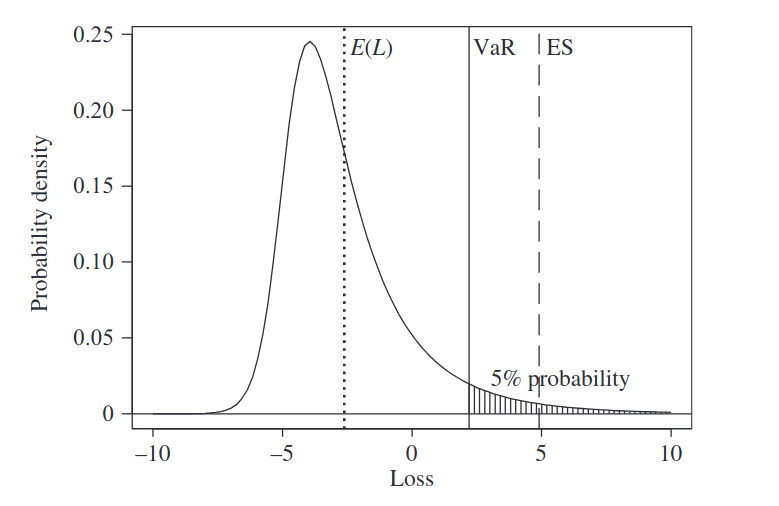
\includegraphics[width=\linewidth]{../img/VaR_CVaR_graph_theory.png}
  \caption{Illustration of $VaR_{0.95}$ and $CVaR_{0.95}$ (where $CVaR_{0.95}$ is labeled as ES). Image sourced from \cite[Figure 2.2.]{mcneil2015quantitative}. \textcolor{red}{TODO: generate the figure myself}}
  \label{fig:VaR_CVaR_graph_theory}
\end{figure}


Value at risk also comes with several advantages and disadvantages. While it is simple to understand and globally accepted by regulators, it is not coherent in general (the subadditivity requirement is not fulfilled), it doesn't quantify the losses exceeding $VaR_{\alpha}(x)$ and it is not convex (this makes it hard to optimize a portfolio with regard to value at risk).

Due to the aforementioned disadvantages of value at risk, another risk measure was considered.
Considering the expected loss exceeding the $VaR_{\alpha}(x)$ level leads to the notion of \textit{Conditional value at risk}. \todo{Add conditional value at risk.}

\begin{defn}{Conditional value at risk} 
\label{cvar_definition}
\\  
\cite[p. 275]{cornuejols_tutuncu_2006}
\\
Let $\alpha$ be the chosen confidence level and let $\mathcal{L}(x,\Upsilon)$ have the meaning of loss distribution as defined above and assume that $\mathbb{E}(\abs{\mathcal{L}(x,\Upsilon)})<\infty$. Then the conditional value at risk or expected shortfall $CVaR_{\alpha}(x)$ is defined as
\begin{equation}
CVaR_{\alpha}(x)=\frac{1}{1-\alpha}\int_{f(x,y) \geq VaR_{\alpha}(x)} f(x,y)p(y) \, \mathrm{d} y.
\end{equation}
\end{defn}
Compared to value at risk, conditional value at risk is a coherent risk measure (for the proof, see \cite[Example 2.26.]{mcneil2015quantitative}), but since value at risk is present in its definition, optimizing a portfolio with regard to conditional value at risk according to this definition suffers from many of the same problems as optimizing a portfolio with regard to value at risk. Therefore, a new method has been developed in \cite{Rockafellar2000OptimizationOC} that allows optimization of conditional value at risk without computing value at risk using linear programming.

\section{Minimising CVaR using scenarios}
In this section, we closely follow the exposition provided in \cite[p. 275-278]{cornuejols_tutuncu_2006}.
Let
\begin{equation}
\label{eq:cvar_approx}
F_{\alpha}(x,\gamma)=\gamma + \frac{1}{1-\alpha} \int_{f(x,y) \geq \gamma} (f(x,y)-\gamma)p(y) \, \mathrm{d}y.
\end{equation}
The function $F_{\alpha}(x,\gamma)$ has three important properties:
\begin{lemma}{Properties of $F_{\alpha}(x,\gamma)$ \cite[p. 276]{cornuejols_tutuncu_2006}.}
\label{lemma:properties_of_cvar_approx} 
\\
The following three properties hold for $F_{\alpha}(x,\gamma)$:
\begin{enumerate}
	\item It is a convex function of $\gamma$.
	\item $VaR_{\alpha}(x)=\underset{\gamma}{\mathrm{argmin}} \, F_{\alpha}(x,\gamma)$.
	\item $ CVaR_{\alpha}(x) = \underset{\gamma}{\mathrm{min}} \, F_{\alpha}(x,\gamma)$.
\end{enumerate}
\end{lemma}
\begin{proof}
For the proof, see \cite[Theorems 1 and 2]{Rockafellar2000OptimizationOC}
\end{proof}
\subsection{CVaR formulation}
If we want to choose a portfolio $x$ that minimises $CVaR_{\alpha}(x)$, we can now do so by minimising $F_{\alpha}(x,\gamma)$ over $x \in \mathcal{X}$ and $\gamma \in \R$ (where $\mathcal{X}$ is some set of portfolios) thanks to the third property in Lemma \ref{lemma:properties_of_cvar_approx}. Of course, Equation \ref{eq:cvar_approx} is not particularly suitable for numerical computations. In practice, as was explained in detail in Chapter \ref{chap1}, the distribution of $\Upsilon$ is approximated using scenarios $\gamma_s$ with associated probabilities $p_s, s=1,\dots,S$.

We can then calculate an approximation of $F_{\alpha}(x,\gamma)$ as
\begin{equation}
\label{eq:cvar_approx_approx}
\hat{F}_{\alpha}(x,\gamma)=\gamma + \frac{1}{1-\alpha} \sum_{s=1}^S  p_s \max (f(x,\gamma_s)- \gamma,0).
\end{equation}
We have arrived at the optimization problem
\begin{equation}
\label{eq:cvar_optim_first}
\underset{x \in \mathcal{X}, \gamma}{\min} \hat{F}_{\alpha}(x,\gamma)= \underset{x \in \mathcal{X}, \gamma}{\min} \gamma + \frac{1}{1-\alpha} \sum_{s=1}^S p_s \max (f(x,\gamma_s)-\gamma,0).
\end{equation}
A trick can be used to turn Equation \ref{eq:cvar_optim_first} into a linear programming problem. If we create new variables $z_s \geq 0$ such that $z_s \geq f(x,\gamma_s)-\gamma$, we can write:
\begin{alignat}{10}
& \underset{x \in \mathcal{X}, z_s \geq 0, \gamma}{\min}  \, \, \, && \gamma + \frac{1}{1-\alpha} \sum_{s=1}^S p_s z_s \\
&s.t. && \, z_s \geq f(x,\gamma_s)-\gamma, s=1,\dots,S
\end{alignat}
which is a linear programming problem.
\subsection{Mean-CVaR formulation}
In this section, we present a more precise formulation for practical use adopted from \cite{cvar_robust_mean_cvar_portfolio_optimization}, particularly when we want to choose a portfolio that minimises the conditional value at risk and also allows for controlling the minimum expected return or setting the degree of risk aversion.
\subsubsection*{Formulation with minimum expected return}
Let $x=(x_1,\dots,x_n)$ be a vector denoting of weights of each of $n$ assets in a portfolio and consider that $\mu=(\mu_1,\dots,\mu_n)$ is a random vector representing the returns of the assets. Consider $S$ scenarios, each with probability $p_s$ and let $r_s = (r_{1,s},\dots,r_{n,s})$ be the particular realisation of $\mu$ in scenario $s$ and let $r_0$ be the minimum required expected return. For simplicity, we do not allow short selling (condition $x_i \geq 0, i=1,\dots,n$). Then we can write
\begin{alignat}{10}
& \underset{x_i \geq 0 , z_s \geq 0, \gamma}{\min}  \, \, \, && \gamma + \frac{1}{(1-\alpha)} \sum_{s=1}^S p_s z_s, \label{cvar_expected_return}  \\
&s.t. && \, z_s \geq  -\sum_{i=1}^{n} x_i r_{i,s} -\gamma, s=1,\dots,S, \nonumber \\
&  && \sum_{i=1}^{n} x_i \bar{R_i} \geq r_0, \label{eq:cvar_expected_return:min_return_equation} \\
&  && \sum_{i=1}^{n} x_i = 1, \nonumber
\end{alignat}
where $\bar{R_i}=\sum_{s=1}^{S}p_s r_{i,s}$, which is still a linear programming problem. Equation \ref{eq:cvar_expected_return:min_return_equation} assures the minimal expected return.
\subsubsection*{Formulation using risk aversion}
Another equivalent formulation might be useful when the decision maker does not require a minimum expected return explicitly, but rather wants to set his risk aversion expectations. This can be achieved by introducing a risk aversion parameter $\lambda \geq 0$ and writing
\begin{alignat}{10}
& \underset{x_i \geq 0 , z_s \geq 0, \gamma}{\min}  \, \, \, && \sum_{i=1}^{n} x_i \bar{R_i} + \lambda \left( \gamma + \frac{1}{(1-\alpha)} \sum_{s=1}^S p_s z_s \right), \label{eq:cvar_risk_aversion} \\
&s.t. && \, z_s \geq  -\sum_{i=1}^{n} x_i r_{i,s} -\gamma, s=1,\dots,S, \nonumber \\
&  && \sum_{i=1}^{n} x_i = 1. \nonumber
\end{alignat}
\section{Minimising CVaR using scenarios in multistage setting}
In the multistage setting, the problem is a bit more complicated. Since the returns now do not occur at one single time but rather it is a sequence of returns, the notion of a risk measure must be extended accordingly. For the purposes of this thesis, we focus on the \textit{end of horizon $CVaR$}, for more advanced topics such as \textit{Nested $CVaR$ model} or \textit{Sum of $CVaR$ model}, we refer the reader to the summary in \cite[Section 1.4.]{kozmikv_phdthesis}.

\subsection{End of horizon CVaR}

\begin{defn}{End of horizon $CVaR$.} \\
Consider Definition \ref{cvar_definition}. If we consider the $CVaR$ calculated from the last stage (at the end of the investment horizon), we call it end of horizon $CVaR$.
\end{defn}
The definition of \textit{end of horizon $CVaR$} is very similar to the definition of regular $CVaR$, with the small difference that the multistage formulation now allows the decision maker to reallocate funds during the investment period (at the end of each stage). 

\subsubsection{End of horizon CVaR - scenario formulation}
We now extend Formulations \ref{cvar_expected_return} and \ref{eq:cvar_risk_aversion} to the multistage case. Consider we want to optimise a portfolio consisting of $n$ stocks over $T$ stages and consider a scenario tree with $S$ leaves (here we abuse notation and write sets $S=\{1,\dots,S\}$, $T=\{1,\dots,T\}$ and $I=\{1,\dots,n\})$. The problem \ref{cvar_expected_return} can then be reformulated as Equation \ref{eq:cvar_multistage_expected_return} by introducing variables $w_{t,s}$ which represent the wealth in scenario $s$ at time $t$ and $tot_s$ which is the total return in scenario $s$.

\begin{alignat}{10}
& \min \, \, \, && \gamma + \frac{1}{(1-\alpha)} \sum_{s=1}^S p_s z_s, \label{eq:cvar_multistage_expected_return}  \\
&s.t. && \, z_s \geq  -tot_s -\gamma, \forall s \in S \nonumber \\
&  && \sum_{s=1}^{S} p_s tot_s \geq r_0, \nonumber \\
& && w_{1,s}=1, \forall s \in S, \nonumber \\
& && w_{t,s}=\sum_{i=1}^{n} x_{i,t,s}, \forall s \in S, \forall t \in \{1,\dots,T-1\}, \label{eq:cvar_multistage_expected_return:wealth_distribution} \\
& && w_{t+1,s}=\sum_{i=1}^{n} r_{i,t,s} x_{i,t,s}, \forall s \in S, \forall t \in \{1,\dots ,T-1\}, \label{eq:cvar_multistage_expected_return:wealth_increases} \\
& && tot_s = \frac{w_{T,s}}{w_{1,s}}, \forall s \in S, \nonumber \\
& && z_s \geq 0, \forall s \in S, \nonumber \\
& && x_{i,t,s} \geq 0, \forall s \in S, \forall i \in I, \forall t \in \{1,\dots ,T-1\}, \nonumber \\
& && \gamma \in \R ,\nonumber \\
& && + \mathrm{nonanticipativity \, constraints}, \nonumber
\end{alignat}
The initial wealth $w_{1,s}$ is set to 1 and in each stage, the wealth increases by the returns obtained in the previous stage (Equation \ref{eq:cvar_multistage_expected_return:wealth_increases}) and is distributed again (Equation \ref{eq:cvar_multistage_expected_return:wealth_distribution}, at the end of the investment horizon we do not need to distribute the wealth into assets again). $r_{i,t,s}$ is the return obtained from stock $i$ at stage $t$ in scenario $s$ (we consider returns indexed by $t$ to occur at the end of stage $t$ (after the portfolio allocations $x_{i,t,s}$ are set), so that Equation \ref{eq:cvar_multistage_expected_return:wealth_increases} makes sense). The returns $r_{i,t,s}$ are of the form $1+r$ (where if the asset gained 6 percent, then $r_{i,t,s}=1.06$). This justifies Equation \ref{eq:cvar_multistage_expected_return:wealth_increases}. $tot_s \, \forall s \in S$ and $r_0$ are then again of the form $1+r$.

\begin{rem}
We do not include the nonanticipativity constraints in the above formulation, since they must be specified explicitly according to the structure of the scenario tree. To illustrate the explicit formulation of nonanticipativity constraints, consider Figure \ref{fig:balanced_scenario_tree}. In the context of the above problem, there are 6 scenarios ($111, 112, 113, 121, 122, 123$). For this illustration, let $\mathbf{x}_{t,s}$ be the vector of allocations to each assets at time $t$ and in scenario $s$. The nonanticipativity constraints now read:
\begin{alignat}{10}
& && \mathbf{x}_{t1,111}=\mathbf{x}_{t1,112}=\mathbf{x}_{t1,113}=\mathbf{x}_{t1,121}=\mathbf{x}_{t1,122}=\mathbf{x}_{t1,123} \nonumber \\
& && \mathbf{x}_{t2,111}=\mathbf{x}_{t2,112}=\mathbf{x}_{t2,113},\mathbf{x}_{t2,121}=\mathbf{x}_{t2,122}=\mathbf{x}_{t2,123}. \nonumber
\end{alignat}
\end{rem}
Similarly, the problem \ref{eq:cvar_risk_aversion} can then be reformulated as Equation \ref{eq:cvar_multistage_risk_aversion}:

\begin{alignat}{10}
& \min  \, \, \, &&\sum_{s=1}^{S} p_s tot_s + \lambda \left( \gamma + \frac{1}{(1-\alpha)} \sum_{s=1}^S p_s z_s \right), \label{eq:cvar_multistage_risk_aversion}  \\
&s.t. && \, z_s \geq  -tot_s -\gamma, \forall s \in S \nonumber \\
& && w_{1,s}=1, \forall s \in S, \nonumber \\
& && w_{t,s}=\sum_{i=1}^{n} x_{i,t,s}, \forall s \in S, \forall t \in \{1,\dots ,T-1\}, \label{eq:cvar_multistage_expected_return:wealth_distribution_risk_aversion} \\
& && w_{t+1,s}=\sum_{i=1}^{n} r_{i,t,s} x_{i,t,s}, \forall s \in S, \forall t \in \{1,\dots ,T-1\}, \label{eq:cvar_multistage_expected_return:wealth_increases_risk_aversion} \\
& && tot_s = \frac{w_{T,s}}{w_{1,s}}, \forall s \in S, \nonumber \\
& && z_s \geq 0, \forall s \in S, \nonumber \\
& && x_{i,t,s} \geq 0, \forall s \in S, \forall i \in I, \forall t \in \{1,\dots ,T-1\}, \nonumber \\
& && \gamma \in \R ,\nonumber \\
& && + \mathrm{nonanticipativity \, constraints}, \nonumber
\end{alignat}
where $\lambda \geq 0$ is a risk aversion parameter and the nonanticipativity constraints would again need to be provided explicitly according to the structure of the scenario tree.
\chapter{Reinforcement learning}
\label{chapter3}
Reinforcement learning is a machine learning paradigm inspired by the natural learning process of humans -- learning by interacting with an environment. All actions we take in our daily lives are in some way punished or rewarded. 
	
For an example, consider touching a hot stove. An immediate negative reward (pain) is received and one learns quickly not to do it again. On the other hand, eating something sweet usually produces a feeling of pleasure (positive reward) and that makes us want to eat more sweets. 

Reinforcement learning methods work in pretty much the same way: an agent is placed in an artificial environment and based on the actions it takes, it receives rewards (positive or negative) and learns to perform the actions that yield the most positive rewards. This is in constrast to the other machine learning paradigms (supervised and unsupervised learning), where no environment exists and the model is taught by minimising some kind of loss over a given dataset. 

In the recent years, machine learning has seen a large surge in activity due to rising computational power and this has not avoided the field of reinforcement learning. Many large institutions and corporations have built teams that specialise in reinforcement learning and have produced groundbreaking results in many disciplines, ranging from beating the best player in the world in the game of Go (see \cite{alphago_paper}), solving the protein folding problem (see \cite{alphafold}), beating some of the best teams in Dota 2 (see \cite{openaifive}) or most recently, finding a faster matrix multiplication algorithm than current state of the art (see \cite{matrix_multiplication}).

In this chapter, we aim to provide the necessary exposition of reinforcement learning methods used in the computational part of this thesis. We mainly follow \cite{sutton2018reinforcement}.

\section{Basic definitions}
As we mentioned, the agent operates in an environment. The agent is aware of the environment and based on the current state of the environment chooses an action. The action is usually chosen as the action that maximises the expected cumulative reward (this may not always be the case, as choosing a less optimal action might be beneficial, we will touch on this in Section \ref{section:explo_vs_exploit}). After the agent performs an action, the state of the environment changes and the agent receives a reward. This happens in a sequence of discrete timesteps until a terminal state of the environment is reached (i.e., if the last chosen action led to winning/losing in the game of chess). One iteration of solving an environment from the initial to the terminal state is called an \textit{episode}. This is best illustrated by the chart that can be found in almost all reinforcement learning books, see Figure \ref{fig:agent_environment_interaction}.

\begin{figure}
  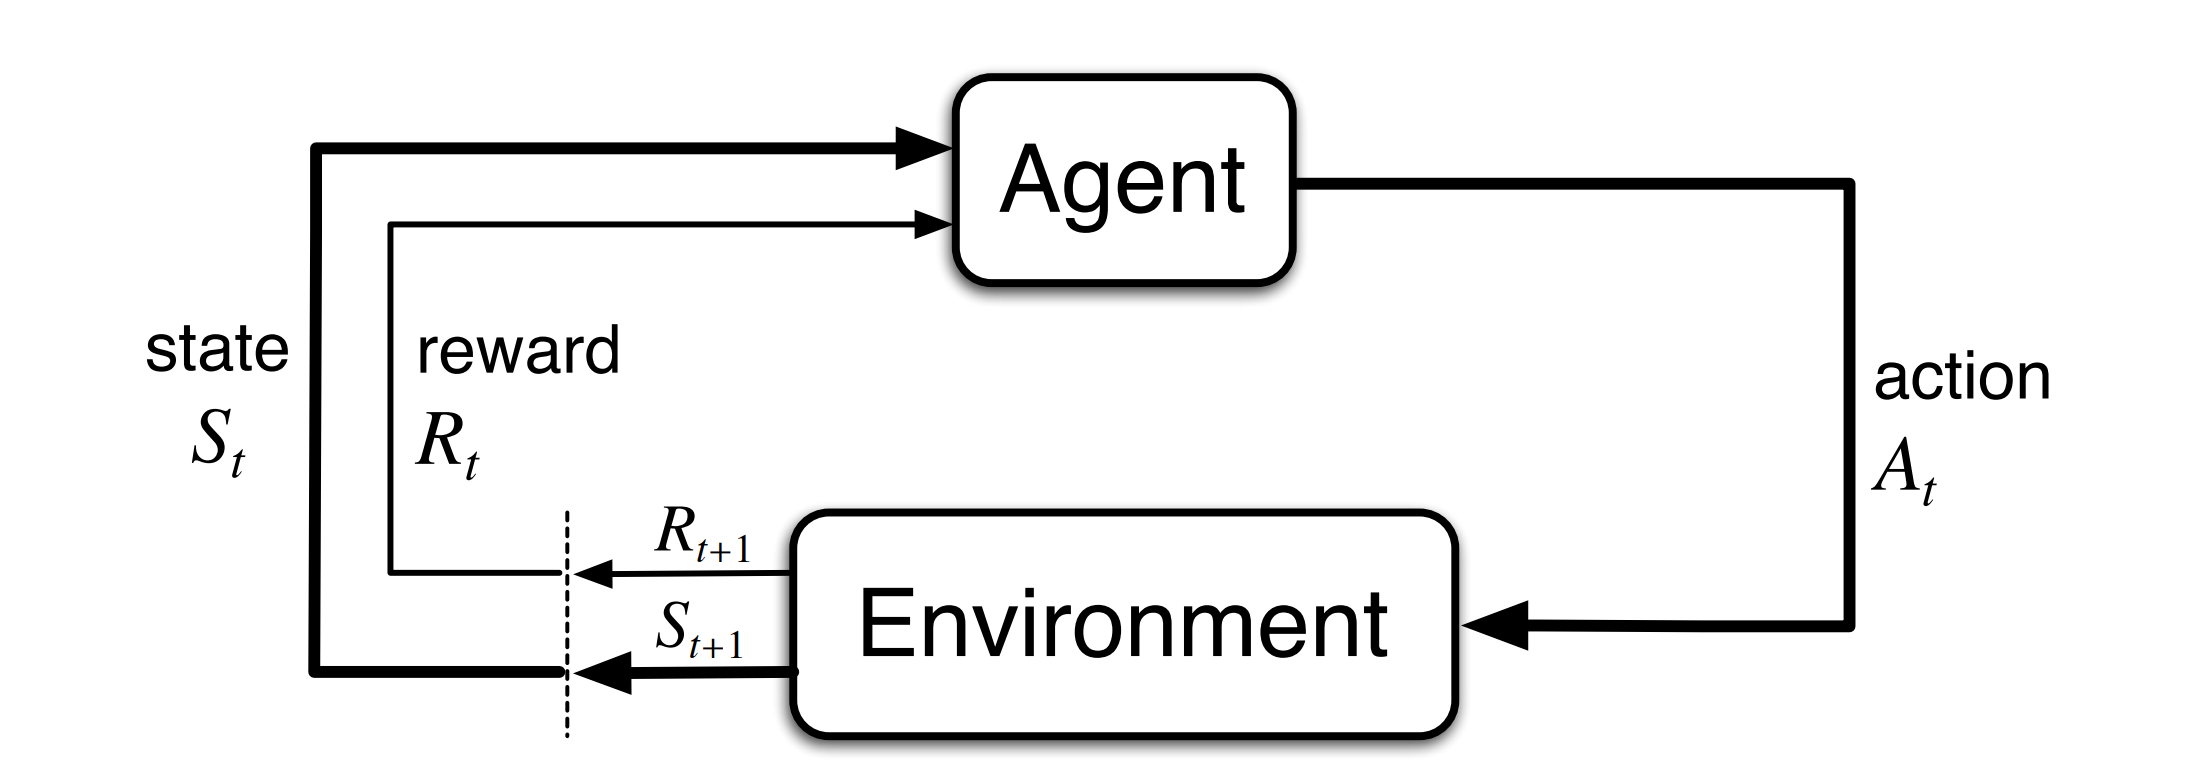
\includegraphics[width=\linewidth]{../img/agent_environment_interaction.png}
  \caption{Illustration of the agent environment interaction. Agent is in state $S_t$ and received reward $R_t$ for the last chosen action $A_{t-1}$, then $A_t$ is chosen by the agent and new state $S_{t+1}$ and reward $R_{t+1}$ are obtained. Image sourced from \cite[Figure 3.1.]{sutton2018reinforcement}.}
  \label{fig:agent_environment_interaction}
\end{figure}

We now introduce the notion of a \textit{Markov decision process}, which is a formalisation of the agent environment interaction discussed above. The following is heavily inspired by \cite[Chapter 3]{sutton2018reinforcement}
\begin{defn}{Markov decision process} 
\label{defn:markov_decision_process}
\\
\cite[Chapter 3]{sutton2018reinforcement}

A Markov decision process is a 5-tuple $(\mathcal{S}, \mathcal{A}, \mathcal{P}, \mathcal{R}, \gamma)$, where 
\begin{enumerate}
\item $\mathcal{S}$ is the set of all possible states,
\item $\mathcal{A}$ is the set of all possible actions,
\item $\mathcal{P}(s_{t+1}|s_{t},a_t)=P(S_{t+1}=s_{t+1}|S_t=s_{t},A_t=a_t)$ is the probability that choosing action $a_t$ in state $s_t$ yields state $s_{t+1}$,
\item $\mathcal{R}(s_t, a_t)=R_{t+1}(S_t=s_t, A_t=a_t)$ is the reward received by choosing action $a_t$ in state $s_t$,
\item $\gamma \in [0,1)$ is the discount factor,

\end{enumerate}
\end{defn}
where $S_t$, $A_t$ and $R_t$ are random variables representing the state, action and reward at timestep $t$. The name Markov decision process is not a coincidence and is related to the Markovian property. Notice that the state transition probabilities depend only on previous state and chosen action and not on the preceeding history. This means that the state must contain all information and no information is carried by the previously visited states and taken actions. Of course, this is a simplification and does not hold in real life (for example, the history of moves can hold information about the strength of an opponent in the game of chess), but it suffices to model even complex phenomena and allows for precise mathematical treatment. 

The agent chooses an action based on the current state to maximise the expected cumulative reward. A function that maps states to probabilities of actions is termed \textit{policy}, see Definition \ref{defn:policy}.

\begin{defn}{Policy} \label{defn:policy}
\\
\cite[Section 3.5]{sutton2018reinforcement} \\
Let $s \in \mathcal{S}$ and $a \in \mathcal{A}$. Then the policy is defined as
\begin{equation*}
\pi(a|s)=P(A_t=a|S_t=s).
\end{equation*}
\end{defn} 
Another fundamental concept is the value function, see Definition \ref{defn:value_function}.

\begin{defn}{Value function} \label{defn:value_function}
\\
\cite[Section 3.5]{sutton2018reinforcement}
\\
Let $\pi$ be a policy and $s \in \mathcal{S}$. Then we define the value function $v_{\pi}(s)$ as
\begin{equation*}
v_{\pi}(s)=\mathbb{E}_{\pi} \left[ \sum_{k=0}^{\infty} \gamma^k R_{t+k+1} | S_t=s \right],
\end{equation*}
\end{defn}
where the subscript $\pi$ in $\mathbb{E}_{\pi}$ refers to the fact that the agent acts according to policy $\pi$.
The value function assigns each state the expected cumulative discounted reward -- the reward that the agent may expect to gain from state $s_t$ into the future. The discount factor $\gamma$ weights the future rewards by how far into the future they may be attained.

Another related notion is the \textit{action value function}, see Definition \ref{defn:action_value_function}.

\begin{defn}{Action value function} \label{defn:action_value_function}
\\
\cite[Section 3.5]{sutton2018reinforcement}
\\
Let $\pi$ be a policy and $s \in \mathcal{S}$ and $a \in \mathcal{A}$. Then we define the action value function $q_{\pi}(s,a)$ as
\begin{equation*}
 q_{\pi}(s,a)=\mathbb{E}_{\pi} \left[ \sum_{k=0}^{\infty} \gamma^k R_{t+k+1} | S_t=s, A_t=a \right].
\end{equation*}
\end{defn}
The action value function is much the same as value function, but it maps the actions taken in a state to the expected cumulative discounted reward rather than just states. The action value function allows the agent to not always take the immediate most rewarding (greedy) action, but rather optimise the reward while taking into account the possible following states and actions. 

The value function and action value functions must be learned by exploring the environment. Unfortunately, the plethora of theory about estimation of these functions (e.g. using the Bellman equations) is out of scope of this thesis. We refer the interested reader to \cite[Section 3.5.]{sutton2018reinforcement} and the references therein.

Another related notion, which builds on the definitions given above is the \textit{advantage function}, see Defintion \ref{defn:advantage_function}.
\begin{defn}{Advantage function} \label{defn:advantage_function}
\\
\cite[Section 3]{a3c_paper}
\\
Let $\pi$ be a policy and $s \in \mathcal{S}$ and $a \in \mathcal{A}$. Denote the value function as $v_{\pi}(s)$ and the action value function as $q_{\pi}(s,a)$. Then we define the advantage function  as
\begin{equation*}
 A_{\pi}(s,a) = q_{\pi}(s,a) - v_{\pi}(s).
\end{equation*}
\end{defn}
The advantage represents the gain that is obtained by taking action $a$ in state $s$ compared to following policy $\pi$.

Our aim is to obtain a policy that maximises the expected cumulative discounted reward. We thus define the \textit{optimal policy}, \textit{optimal value function} and \textit{optimal action value function}, see Definition \ref{defn:optimal_definitions}.

\begin{defn}{Optimal policy, value function and action value function} 
\label{defn:optimal_definitions} 
\\
\cite[Section 3.6]{sutton2018reinforcement}
\\
Let $R(\pi)$ be the expected cumulative discounted reward obtained by following policy $\pi$. Then we define the optimal policy as
\begin{equation*}
 	\pi^* = \underset{\pi}{argmax} \, R(\pi).
\end{equation*}
Similarly, the optimal value function and optimal action value function are given by: 
\begin{equation*}
 	v^*(s) = \underset{\pi}{\max} \, v_{\pi}(s)
\end{equation*}
and
\begin{equation*}
 	q^*(s,a) = \underset{\pi}{\max} \, q_{\pi}(s,a).
\end{equation*}
respectively for $s \in \mathcal{S}$ and $a \in \mathcal{A}$.
\end{defn}

\section{Exploration vs exploitation}
\label{section:explo_vs_exploit}
The optimal policy, value function and action value function must be learned by interacting with the environment. The agent now faces a dillema -- either to maximise his known reward (act greedily, but potentially get stuck with a policy that is not optimal) or explore the environment and update the policy in order to get the (globally) optimal policy. This exploration-exploitation tradeoff is always present with reinforcement learning and many approaches for dealing with it exist. An example are the $\epsilon$-greedy methods, where the agent acts greedily $(1-\epsilon) \, \%$ of the time and performs a random action $\epsilon \, \%$ of the time. $\epsilon$ is usually set to a value close to 1 at the beginning of training and decreased over time, the final threshold at which $\epsilon$ is kept constant is usually somewhere in $[0,0.1]$. For more information, we refer the reader to \cite[Section 2.7.]{sutton2018reinforcement}.

\section{Algorithm classes}
In this section, we aim to present a basic summary of current reinforcement learning methods with particular focus on policy-gradient methods.
\subsection{Model free vs. model based algorithms}
The most fundamental dividing line between reinforcement learning algorithms is whether the agent is given a model of the environment which allows the agent to take into account future states before they are experienced. The model is represented by the state transition function $\mathcal{P}$ as defined in Definition \ref{defn:markov_decision_process}. Having the model in hand obviously helps the agent learn tremendously, but having such a model in practice is quite rare, thus the model free methods are being used much more extensively. We focus on model free algorithms in this text.

\subsection{Model free methods}
In comparison to model based methods, the model free methods learn by trial and error.
Examples of these methods are e.g. Monte Carlo Sampling, SARSA, Q-learning, Actor critic, Proximal policy optimization (PPO) and Trust region policy optimization (TRPO). These methods can be divided into two groups -- value based methods and policy based methods. In this thesis, we focus particularly on the Proximal policy optimization method (as it will be used in the computational part of this thesis for reasons explained later), but we also give an introduction to Q learning, as it helps with understanding of how deep neural networks are used in the field of reinforcement learning, the Actor critic architecture and the Trust region policy optimization. We assume that the reader is familiar with basics of deep learning (such as architecture of neural networks and basic algorithms for training them such as stochastic gradient descent), a great introduction can be found in \cite[Part 2]{deep_learning_book}.
\subsubsection{Value based methods}
\subsubsection{$Q$ learning}
In this section, we follow \cite[Section 6.5.]{sutton2018reinforcement}.
The most famous example of a value based method is $Q$ learning.
Let $q^*(s,a)$ denote the optimal action value function as defined in Definition \ref{defn:optimal_definitions} and let $Q(s,a)$ be an estimate of $q^*(s,a), s \in \mathcal{S}, a \in \mathcal{A}$. If the sets $\mathcal{S}$ and $\mathcal{A}$ are finite, then the values of $Q(s,a)$ can be represented by a table and updated according to the updating rule presented in Equation \ref{eq:q_learning_updating_rule}.

\begin{equation}
Q(s_t, a_t) \leftarrow Q(s_t, a_t) + \varphi \left[r_{t+1} + \gamma \underset{a \in \mathcal{A}}{\max}Q(s_{t+1}, a) - Q(s_t, a_t) \right],
\label{eq:q_learning_updating_rule}
\end{equation}
where $\varphi$ is the learning rate, $\gamma$ is the discount factor, $s_t, a_t$ are the current state and current chosen action respectively, $s_{t+1}$ is the next state following action $a_t$, $r_{t+1}$ is the reward obtained by choosing action $a_t$ and the subscript $t$ is added to emphasize the transition between current and next step.
The whole algorithm can be summarised as follows:

\renewcommand{\algorithmicrequire}{\textbf{Input:}}
\renewcommand{\algorithmicensure}{\textbf{Output:}}


\begin{algorithm}[H]
\small
\caption{Vanilla Q-learning \cite[p. 131]{sutton2018reinforcement}}\label{alg:q_learning}
\begin{algorithmic}
\Require{Choose the learning rate $\varphi \in (0,1]$ and exploration parameter $\epsilon>0$, number of episodes, initialise $Q(s, a) \, \mathrm{randomly}, s \in \{s \, \mathrm{for} \,  s \, \mathrm{in} \, \mathcal{S} \, \mathrm{if} \, s \, \mathrm{is \, not \, terminal}\}$ and $Q(s,a)=0$ for $s$ terminal, $a \in \mathcal{A}$ (terminal state of the environment means that the episode is finished).}
\For{episode in $\{$1,...,number of episodes$\}$}
\State $s_t \leftarrow s_0$ Reset environment state 
\While{$s_t$ is not terminal}
\State $a_t \leftarrow$ Choose action $a_t$ using an epsilon-greedy policy according to $Q(s_t,\cdot).$
\State $s_{t+1}, r_{t+1} \leftarrow$ act on action $a_t$, obtain new state $s_{t+1}$ and reward $r_{t+1} $
\State Update $Q(s_t,a_t)$ using Equation \ref{eq:q_learning_updating_rule}
\State $s_t \leftarrow s_{t+1}$
\EndWhile
\EndFor
\end{algorithmic}
\end{algorithm}
It has been shown that under the assumption that all state-action pairs continue to be updated during training, then $Q$ converges to $q^*$ almost surely \cite[p. 131]{sutton2018reinforcement}. This variant of $Q$-learning has an obvious problem -- it depends on a table for keeping the values of the $Q$ function and thus does not generalise to complex state spaces (such as infinite ones). To tackle this problem, a neural network has been introduced in place of the $Q(s,a)$ table as a function approximator, which we can then write as $Q(s,a;\theta)$, where $\theta$ are the weights of the neural network. This approach has been popularised by \cite{deep_q_learning_paper}, where they used $Q$-learning along with a neural network as a function approximator (and many other particular improvements such as experience replay, that are unfortunately out of the scope of this thesis) to achieve superhuman performance on several Atari 2600 games. The reader interested in deep $Q$-learning can find the algorithm in \cite[Algorithm 1]{deep_q_learning_paper}.

\subsubsection{Policy approximation methods}
The theory of value based methods assumed that we estimate the value function and action value function and then based on them somehow choose the policy (such as taking the action with maximum value). However, another approach is possible -- modelling the policy explicitly. In this section, we mostly follow  \cite[Chapter 13]{sutton2018reinforcement} and \cite[Section 2]{proximal_policy_optimization}.

Policy approximation methods assume that the policy $\pi(a|s;\theta), a \in \mathcal{A}, s \in \mathcal{S}$ is dependent on parameters $\theta \in \R^d$ where $d \in \N.$ In general, the aim of these methods is to maximise some kind of performance measure $J(\theta)$. The performance measure $J$ is chosen such that the gradient $\nabla_{\theta}J$ exists and by estimating the gradient as $\widehat{\nabla_{\theta_{\tau}} J(\theta_{\tau})}$, the policy can be optimised using stochastic gradient ascent (where the subscript $\tau$ implies that this estimate is computed in the $\tau$-th update in the stochastic gradient ascent process). In practice, $\widehat{\nabla_{\theta_{\tau}} J(\theta_{\tau})}$ is estimated by averaging a batch of samples, we will denote this as $\mathbb{E}_b \widehat{\nabla_{\theta_{\tau}} J(\theta_{\tau})}$ where the symbol $\mathbb{E}_b$ refers to the average of a batch of samples. We can then write the very general update rule

%Equation \ref{eq:policy_approximation_updating_rule}
%
\begin{equation*}
\label{eq:policy_approximation_updating_rule}
\theta_{\tau+1}=\theta_{\tau}+\varphi \mathbb{E}_b\widehat{\nabla_{\theta_{\tau}} J(\theta_{\tau})},
\end{equation*}
where $\varphi$ is the learning rate.
% and $\widehat{\nabla_{\theta_{\tau}} J(\theta_{\tau})}$ is the estimate of the gradient of the performance measure $J$ with respect to $\theta_{\tau}$. 
Due to the aforementioned updating rule, these methods are also often called \textit{policy gradient methods}. 

\begin{rem} 
When using policy approximation methods, we do not need to randomly sample actions $\epsilon \%$ of the time to ensure exploration. All that is needed is to ensure that the policy does not become deterministic. This can be achieved by ensuring that $\pi(a|s;\theta) \in (0,1)$ \cite[Section 13.1]{sutton2018reinforcement}.
\end{rem}

A significant theoretical advantage compared to value based methods is that “\textit{with continuous policy parameterization the action probabilities change smoothly as a function of the learned parameter, whereas in $\epsilon$-greedy selection the action probabilities may change dramatically for an arbitrarily small change in the estimated action values, if that change results in a different action having the maximal value. Largely because of this stronger convergence guarantees are available for policy-gradient methods than for action-value methods}” \cite[Section 13.2]{sutton2018reinforcement}. We refer the reader to the Policy gradient theorem located therein.

There exist also hybrid methods between policy gradient methods and value based methods, where the policy, value function and action value function are all learned -- such methods are called \textit{actor critic} methods.

\subsubsection{Advantage actor critic}
In this section, we present the theory behind the (asynchronous) advantage actor critic (A3C) algorithm as developed in \cite{a3c_paper}, as it shows well the structure of the neural net that is used in the PPO algorithm.

The advantage actor critic is a policy approximation algorithm that learns not only the policy but also the action value function. Let us first decipher the name of the algorithm. Advantage refers to the advantage function defined in Definition \ref{defn:advantage_function}, actor refers to the learned policy approximation and critic refers to the learned action value function approximation (both the actor and the critic are neural networks that are used as function approximators). In practice, the actor and critic networks share some parameters (they can be thought of as a single neural net with diverging structure, such as a first shared layer and then diverging such that the second layer is not shared between the actor and the critic).

Denote the weights of the actor as $\theta$ and weights of the critic as $\theta_v$, thus the estimated policy can be written as $\pi(a|s;\theta)$, $a \in \mathcal{A}, s \in \mathcal{S}$. The performance measure $J$ that A2C maximises can be written as 
\begin{equation*}
\log (\pi(a|s;\theta))\widehat{A}(s,a;\theta,\theta_v),
\end{equation*}
and the gradient of the performance measure can be written as
\begin{equation*}
\mathbb{E}_b \nabla_{\theta'} \log (\pi(a_b|s_b;\theta'))\widehat{A}(s_b,a_b;\theta,\theta_v),
\end{equation*}
where the gradient is taken only with respect to the actor variables affecting the policy (the advantage can be thought of as constant with regard to the differentiation) and where we add the subscript $b$ to $a_b$ and $s_b$ to indicate that they belong to a batch of samples and where $\widehat{A}(s_b,a_b;\theta,\theta_v)$ is the estimated advantage function (for details on how it can be estimated, see \cite[Section 4]{a3c_paper}). Note that this update only updates the policy and not the value function. A different updating scheme is used for the parameters of the critic, where a quadratic error between the estimated value function and observed rewards is minimised, the details can be found in the original paper \cite[Algorithm S3]{a3c_paper}.
% given by 
%\begin{equation}
%\widehat{A_t}(s_t,a_t;\theta,\theta_v)=\sum_{i=0}^{k-1}\gamma^i r_{t+1} + \gamma^k V(s_{t+k};\theta_v) - V(s_{t};\theta_v),
%\end{equation}
%where $\gamma$ is the discount factor and where $k$ is the number of steps the agent has taken before the update, which is upper bounded by a chosen hyperparameter $t_{max}$. $t_{max}$ chooses at most how many steps the agent should take in an environment. 
%The update is performed whenever a final state is reached or when $t_{max}$ steps have been taken.
%\begin{rem}
%Notice that in the formula for $\widehat{A_t}(s_t,a_t;\theta,\theta_v)$ the parameters $\theta$ are not explicitly present. In reality, the rewards $r_{(\cdot)}$ are chosen by the policy and thus depend on the parameters $\theta$. \todo{is this remark correct? please check} 
%\end{rem}

In the original paper, they made use of asynchronous updates to supposedly improve training stability. It was later shown in the paper \cite{a3c_asynchrony_not_necessary} that the asynchronicity provides no added benefit in performance.

\subsection{Trust region policy optimization}
The trust region policy optimization method, developed in \cite{TRPO}, is a special case of policy gradient methods, as it introduces a special constraint on the policy parameters, such that the change in the policy is not too large at each step. This is done by imposing the constraint that the Kullback-Leibler Divergence between the two policies is not too large. The Kullback-Leibler Divergence is defined in Definition \ref{defn:kl_divergence}.
\begin{defn} \label{defn:kl_divergence}
{Kullback-Leibler Divergence}
\\
Let $P$ and $Q$ be discrete random variables with the same support $\mathcal{S}$. Let $P(x)$ and $Q(x)$ denote the probability distribution functions of $P$ and $Q$, $x \in \mathcal{S}$. Then the Kullback-Leibler Divergence, denoted $D_{KL}(P,Q)$ is calculated is
\begin{equation*}
D_{KL}(P,Q) = \mathbb{E}_{P} \log(\frac{P}{Q}) = \sum_{x \in \mathcal{S}} P(x) \log(\frac{P(x)}{Q(x)}),	
\end{equation*}
where the subscript $P$ in $\mathbb{E}_{P}$ denotes that the expectation is taken with respect to the probability distribution of the random variable $P$.
\end{defn}
$D_{KL}$ quantifies the difference between discrete probability distributions. More details can be found in \cite{KL_divergence}.

In practice, $D_{KL}(\pi_{A},\pi_{B})$ between two policies $\pi_{A}$ and $\pi_{B}$ is bounded from above using some parameter $\delta$. At each step, the optimization problem that is being solved to update the policy is given in Equation \ref{eq:TRPO}.
\begin{alignat}{10}
&  \underset{\theta_{\tau+1}}{\max} \, && \mathbb{E}_b \frac{\pi(a_b, s_b|\theta_{\tau+1})}{\pi(a_b, s_b|\theta_{\tau})} \widehat{A}(a_b, s_b) \label{eq:TRPO} \\
s.t. & && \mathbb{E}_b D_{KL}(\pi(\cdot, s_b|\theta_{\tau}), \pi(\cdot, s_b|\theta_{\tau+1})) \leq \delta \nonumber,
\end{alignat}
where $\theta_{\tau+1}$ are the new parameters of the policy after the update and $\widehat{A}(a_b, s_b)$ is an estimate of the advantage function, where again the subscript $b$ is added to imply that $a_b$ and $s_b$ belong to a batch of samples.
The objective function that is maximised here is a local approximation of a quantity that \textit{“represents the expected return
of another policy $\pi(\cdot,\cdot|\theta_{\tau+1})$ in terms of the advantage over $\pi(\cdot,\cdot|\theta_{\tau})$”} \cite[Equation 1]{TRPO}. For details (such as how $\widehat{A}(a_b, s_b)$ is calculated\footnote{which we do not show, as it would require developing needlessly complex notation and it is not particularly relevant for our purposes}), see \cite[Section 2-4]{TRPO}.

\subsection{Proximal policy optimization}
The Proximal policy optimization algorithm (PPO) was developed in \cite{proximal_policy_optimization} by combining a neural network used for estimation of action value function and the policy approximation with the trust region idea (limiting the magnitude of change in KL diveregence) used in TRPO, we follow their exposition. Consider Equation \ref{eq:ppo}.
\todo{Please verify this section is correct - the notation in the literature is kind of rough and I had a hard time bringing it all together to make sense. I think I did so correctly, but it would be great to double check.}

\begin{equation}
\label{eq:ppo}
\footnotesize	
 L_{CLIP}(\theta_{\tau}', \theta_{\tau}) = \min(r(\theta_{\tau}',\theta_{\tau})\widehat{A}(a, s), \, \mathrm{clip}(r(\theta_{\tau}',\theta_{\tau}), 1-\delta, 1+\delta)\widehat{A}(a, s))),
\end{equation}
where $r(\theta_{\tau}',\theta_{\tau}) = \frac{\pi(a, s|\theta_{\tau}')}{\pi(a, s|\theta_{\tau})}$, $\delta$ is a hyperparameter and 
\begin{equation*}
\mathrm{clip}(a, 1-\delta, 1+\delta) = \min(1+\delta, \max(a,1-\delta)), a \in R.
\end{equation*}

The first term in Equation \ref{eq:ppo} is the same as in the objective function of the TRPO method, see Equation \ref{eq:TRPO}. The second term in the minimum clips the ratio $r(\theta_{\tau}',\theta_{\tau})$, which  has the effect of limiting the change of the policy so that the change is not too large (controlled by $\delta$). The minimum in Equation \ref{eq:ppo} is then taken to get a lower bound on the same objective as used in TRPO.

$L_{CLIP}(\theta_{\tau}', \theta_{\tau})$ is then combined with a value function error term $L_{VF}(\theta_{\tau}')$ and potentially also an entropy term (which is omitted in this exposition), giving rise to the following performance measure $L$ as given in \ref{eq:ppo_performance_measure}.

\begin{equation}
\label{eq:ppo_performance_measure}
L(\theta_{\tau}', \theta_{\tau}) =  L_{CLIP}(\theta_{\tau}', \theta_{\tau}) - c_1 L_{VF}(\theta_{\tau}'),
\end{equation}
where $c_1$ is a hyperparameter and $L_{VF}(\theta_{\tau}')=(v_{\theta_{\tau}'}(s)-v^{target})^2$, where $v^{target}$ is the observed cumulative return of the state $s$ obtained during training. This performance measure is then maximised using stochastic gradient ascent (again, the stochastic gradient ascent update is performed using $\mathbb{E}_b \nabla_{\theta_{\tau}'} L(\theta_{\tau}', \theta_{\tau})$, which is the average over a batch of samples). Note that while the parameters $\theta_{\tau}'$ are shared for the policy approximation and the value function approximation $v_{\theta_{\tau}'}$, a similar shared neural net architecture as was used in the actor critic framework can be used here such that only some of the parameters are shared (such as a common first layer). Particularly, A2C is a special case of PPO as was shown in \cite{a2c_ppo_special_case}. 

Empirically, PPO performs better than A2C and TRPO and is more sample efficient (requires less timesteps to reach a given level of performance). Particularly, in a blogpost, OpenAI said that \textit{“it has become the default reinforcement learning algorithm they use due to its ease of use and good performance”}, see \cite{openaiblogpost}.

%The PPO algorithm, written exactly as originally written in \cite{proximal_policy_optimization}, then reads:
%
%\begin{algorithm}[H]
%\small
%\caption{PPO, Actor Critic style \cite[Algorithm 1]{proximal_policy_optimization}} \label{alg:ppo}
%\begin{algorithmic}
%\For{iteration in 1,2,... do}
%	\For{actor in 1,2,...,$N_A$ do}
%		\State Run policy $\pi(\cdot, \cdot|\theta_t)$ in environment for $T$ timesteps
%		\State Compute advantage estimates $\widehat{A}_1,...,\widehat{A}_T$
%	\EndFor
%	\State Optimize $L(\theta_{t+1}, \theta_{t})$ with respect to $\theta_{t+1}$, with $K$ epochs and minibatch 	    \State size $M \leq N_AT$
%	\State $\theta_t \leftarrow \theta_{t+1}	$
%\EndFor
%\end{algorithmic}
%\end{algorithm}


\chapter{It all comes together}



\chapter*{Conclusion}
\addcontentsline{toc}{chapter}{Conclusion}


%%% Bibliography
%%% Bibliography (literature used as a source)
%%%
%%% We employ bibTeX to construct the bibliography. It processes
%%% citations in the text (e.g., the \cite{...} macro) and looks up
%%% relevant entries in the bibliography.bib file.
%%%
%%% The \bibliographystyle command selects, which style will be used
%%% for references from the text. The argument in curly brackets is
%%% the name of the corresponding style file (*.bst). Both styles
%%% mentioned in this template are included in LaTeX distributions.

\bibliographystyle{plainnat}    %% Author (year)
% \bibliographystyle{unsrt}     %% [number]

\renewcommand{\bibname}{Bibliography}

%%% Generate the bibliography. Beware that if you cited no works,
%%% the empty list will be omitted completely.

\bibliography{bibliography}

%%% If case you prefer to write the bibliography manually (without bibTeX),
%%% you can use the following. Please follow the ISO 690 standard and
%%% citation conventions of your field of research.

% \begin{thebibliography}{99}
%
% \bibitem{lamport94}
%   {\sc Lamport,} Leslie.
%   \emph{\LaTeX: A Document Preparation System}.
%   2nd edition.
%   Massachusetts: Addison Wesley, 1994.
%   ISBN 0-201-52983-1.
%
% \end{thebibliography}


%%% Figures used in the thesis (consider if this is needed)
%\listoffigures

%%% Tables used in the thesis (consider if this is needed)
%%% In mathematical theses, it could be better to move the list of tables to the beginning of the thesis.
%\listoftables

%%% Abbreviations used in the thesis, if any, including their explanation
%%% In mathematical theses, it could be better to move the list of abbreviations to the beginning of the thesis.
%\chapwithtoc{List of Abbreviations}

%%% Attachments to the master thesis, if any. Each attachment must be
%%% referred to at least once from the text of the thesis. Attachments
%%% are numbered.
%%%
%%% The printed version should preferably contain attachments, which can be
%%% read (additional tables and charts, supplementary text, examples of
%%% program output, etc.). The electronic version is more suited for attachments
%%% which will likely be used in an electronic form rather than read (program
%%% source code, data files, interactive charts, etc.). Electronic attachments
%%% should be uploaded to SIS and optionally also included in the thesis on a~CD/DVD.
%%% Allowed file formats are specified in provision of the rector no. 72/2017.
\appendix
\chapter{Attachments}

\section{First Attachment}
\begin{center}
\begin{table}[H]
\centering
\begin{tabular}{lllllll}
\toprule
        &     &      &      &      &      \\
 ACGL &   AFL &  AIG &   AJG &   ALL &   AON &   AXP \\
  BAC &   BEN &   BK &   BLK &   BRO &     C &    CB \\
 CINF &   CMA &  COF &   FDS &  FITB &    GL &    GS \\
 HBAN &   HIG &  IVZ &   JPM &   KEY &     L &   LNC \\
   MCO &   MMC &   MS &   MTB &  NTRS &   PGR &   PNC \\
   RE &    RF &  RJF &  SCHW &  SIVB &  SPGI &   STT \\
   TFC &  TROW &  TRV &   USB &   WFC &   WRB &  ZION \\
   \bottomrule
\end{tabular}
\caption{Stock tickers used in Chapter \ref{chapter4}.}
\label{table:stock_tickers_used}
\end{table}

\begin{table}[H]
\centering
\begin{tabular}{llllll}
\toprule
ALL &   BK &  ACGL &  FDS &  ZION &  TROW \\
 STT &  RJF &  SPGI &  AON &   LNC &   USB \\
 AXP &  AIG &   AJG &  BLK &    RE &  SIVB \\
 NTRS &   CB &   WRB &  BRO &     L &   IVZ \\
  BAC &   GS &   WFC &  MTB &   MMC &   BEN \\
  \bottomrule
\end{tabular}
\caption{Stock tickers in set $A$.}
\label{table:stock_tickers_in_set_A}
\end{table}


\begin{table}[H]
\centering
\begin{tabular}{llll}
\toprule
 HBAN &   COF &  JPM &  AFL \\
 PGR &   CMA &   RF &  TFC \\
 CINF &   MCO &   MS &    C \\
  HIG &  FITB &  TRV &   GL \\
 SCHW &   PNC &  KEY &     \\
 \bottomrule
\end{tabular}
\caption{Stock tickers in set $B$.}
\label{table:stock_tickers_in_set_B}
\end{table}



\end{center}




\openright
\end{document}
